%%% Local Variables:
%%% mode: Xelatex
%%% TeX-master: t
%%% End:

\documentclass[draftformat,mathCMR]{HUSTthesis}%草稿用这个
%\documentclass[finalformat,mathCMR]{HUSTthesis}%盲审用这个
%\raggedbottom

\usepackage{HUSTtils}% 所有其它可能用到的包都统一放到这里了,可以根据自己的实际添加或者删除。这样做主要是为了避免class文件过于臃肿。
% \setmainfont{Times New Roman}[Scale=.9]
\setmainfont{Times New Roman}
%\includeonly{body/chap02}

\begin{document}

%定义所有的eps文件在 figures 子目录下
\graphicspath{{figures/}}

% 生成封面,版权页,摘要

\frontmatter

%%% Local Variables:
%%% mode: Xelatex
%%% TeX-master: t
%%% End:

\ctitle{标题:宋体,英文 Times New Roman,一号,加粗,不超 30 字\\
\textcolor{red}{中英文标题、学科专业、导师姓名正确、一致}}

\xuehao{D2019xxxxx} \schoolcode{10487}
\csubjectname{XXXXX} \cauthorname{XXX}
\csupervisorname{XXX} \csupervisortitle{教授}
\defencedate{202X~年~X~月~X~日} \grantdate{}
\chair{}%
\firstreviewer{} \secondreviewer{} \thirdreviewer{}

\etitle{English Title,Times New Roman,小二号,实词的首字母大写\\
\textcolor{red}{中英文标题、学科专业、导师姓名正确、一致}}
\edegree{Doctor of Engineering}
\esubject{Control Science and Engineering}
\eauthor{(中文习惯,姓在前且姓全部大写)}
\esupervisor{Prof. xxx}
\edate{May, 2022}

%定义中英文摘要和关键字
\cabstract{

摘要是学位论文极为重要、不可缺少的组成部分,它是论文的窗口,并频繁用于国内外资料交流、情报检索、二次文献编辑等。其性质和要求如下:\par
    [1] 摘要即摘录论文要点,是论文要点不加注释和评论的一篇完整的陈述性短文,具有很强的自含性和独立性,能独立使用和被引用。\par
    [2] 博士学位论文的摘要应包含全文的主要信息,并突出创造性成果。\par
    [3] 内容范围应包含以下基本要素:\par
    \hspace{1em}(1) 目的:研究、研制、调查等的前提、目的和任务以及所涉及的主题范围。\par
    \hspace{1em}(2) 方法:所用原理、理论、条件、对象、材料、工艺、手段、装备、程序等。\par
    \hspace{1em}(3) 结果:实验的、研究的、调查的、观察的结果、数据,被确定的关系,得到的效果、性能等。\par
    \hspace{1em}(4) 结论:结果的分析、研究、比较、评价、应用;提出的问题,今后的课题,建议,预测等。\par
    \hspace{1em}(5) 其他:不属于研究、研制、调查的主要目的,但就其见识和情报价值而言也是重要的信息。\par
    [4] 摘要的详简度视论文的内容、性质而定,\textcolor{red}{博士学位论文摘要一般为800-1000汉字。}\par
    [5] 摘要及全文中均不得出现“我们”等字样。一般不用图、表、化学结构式、计算机程序,不用非公知公用的符号、术语和非法定的计量单位。\par
    [6] 摘要中一般不使用缩写词,若实在需要,在第一次使用前,需给出中文全称(缩写词);在使用英文缩写词之前,需给出中文全称(英文全称,缩写词),再次出现时可以采用中文或英文缩写词。\par
    [7] \textcolor{red}{关键词应有3至8个,另起一行置于摘要下方,领域从大到小排列。关键词之间用分号隔开,最后一个关键词后面无标点。}\par
    [8] 摘要、关键词采用中文宋体;英文Times New Room;小四号;}


\ckeywords{关键词1;关键词2;关键词3}

\eabstract{This is abstract. 

英文摘要字体为Times New Roman,小四,1.5倍行距。

\textcolor{red}{英文摘要和关键词应与中文相对应。}英语摘要用词应准确,使用本学科通用的词汇;摘要中主语(作用)常常省略,因而一般使用被动语态;应使用正确的时态,并要注意主、谓语的一致,必要的冠词不能省略。}

\ekeywords{Keyword1, Keyword2, Keyword3}

\makecover

%目录
\tableofcontents

% 对照表
\begin{denotation}
\item[xue] 我的姓
\item[ruini] 我的名
\item[W.M. Zheng]  我的老师
\item[Tsinghua] 学校名
\item[Long] 来个比较长的,看看会出现什么情况。
\item[劝  学] 君子曰:学不可以已。青,取之于蓝,而青于蓝;冰,水为之,而寒于水。
  木直中绳。(车柔)以为轮,其曲中规。虽有槁暴,不复挺者,(车柔)使之然也。故木
  受绳则直, 金就砺则利,君子博学而日参省乎己,则知明而行无过矣。吾尝终日而思
  矣,  不如须臾之所学也;吾尝(足齐)而望矣,不如登高之博见也。登高而招,臂非加
  长也,  而见者远;  顺风而呼,  声非加疾也,而闻者彰。假舆马者,非利足也,而致
  千里;假舟楫者,非能水也,而绝江河,  君子生非异也,善假于物也。积土成山,风雨
  兴焉;积水成渊,蛟龙生焉;积善成德,而神明自得,圣心备焉。故不积跬步,无以至千
  里;不积小流,无以成江海。骐骥一跃,不能十步;驽马十驾,功在不舍。锲而舍之,朽
  木不折;  锲而不舍,金石可镂。蚓无爪牙之利,筋骨之强,上食埃土,下饮黄泉,用心
  一也。蟹六跪而二螯,非蛇鳝之穴无可寄托者,用心躁也。\pozhehao{} 荀况
\end{denotation}
  

\mainmatter
%%% mode: latex
%%% TeX-master: t
%%% End:

\chapter{模板简介}
\label{cha:intro}

\section{概述}
\label{sec:general intro}
论文页边距、行距全文统一。正文小四,中文宋体、英文Times New Roman, 1.5倍行距,图表五号。
非章节结束,正文页不留白,确有需要留白不超过3行。

本模板为华工博士论文~\LaTeX~模板~3.2
版本,新版本基于清华大学学位论文~\LaTeX+CJK
模板(薛瑞尼版本)和华中科技大学博士学位论文~\LaTeX+CJK 模板1.0
版本。模板作者试图尽量使此模板满足华工研院提出的格式要求~\cite{guide,standard},
但不承诺~100\%
满足,即:存在模板使用者需要在此模板基础上再作修正的可能。
本模板亦可充当一份速查手册,文中包含了尽可能多的各种论文常见元素。
但值得注意的是,在正式的论文写作中,应保持格式上的简洁和风格上的
一致,避免出现种类繁多的元素。

\section{参考资料}
\label{sec:requirement}
本文主要为关于~\LaTeX~模板本身使用方法的介绍,关于毕业论文写作内容上的要求,使用者请参阅《华中科技大学研究生学位论文写作指南》~\cite{guide}、《华中科技大学博士、硕士学位论文撰写规定》~\cite{standard}、《理工科-博士-华中科技大学学位论文参考模板》~\cite{modal}等文档。

模板需要使用者具备基本的~\LaTeX~知识,并有一定的使用能力。
对于一些常见构成元素的使用问题,如表格、图形等,
使用者可查阅~\inlinecite{TEXGURU99, OETIKER02} 等文档。
\section{模板编译简介}
\label{sec:compile}

\subsection{XeLatex}
\label{sec:xelatex}

这种编译模式下执行的命令依次为:
\begin{verbatim}
xelatex main 
bibtex main % 编译参考文献文件 *.bib
xelatex main
\end{verbatim}
注意当文档中的引用信息(ref 和 cite)发生变化后,就至少需要运行~
3 次~latex 命令,从而正确显示交叉引用信息。

\section{模板包含文件简介}
\label{sec:checklist}

\subsection{文件清单}

表~\ref{tab:template-files} 列举了本模板主要文件及其功
能。
\begin{table}[htb]
  \centering
  \caption{模板文件清单}
  \label{tab:template-files}
  \begin{minipage}[t]{0.8\linewidth} % 如果想在表格中使用脚注,minipage是个不错的办法
    \begin{tabular*}{\linewidth}{m{3cm}m{10cm}}
      \toprule[1.5pt]
      {\hei 文件名}  & {\hei 描述} \\\midrule[1pt]
      HUSTthesis.cls & 模板类文件\\
      HUSTbib.bst    & 参考文献~Bib\TeX{} 样式文件\\
      HUSTtils.sty   & 常用的包和命令写在这里,减轻主文件的负担\\
      \bottomrule[1.5pt]
    \end{tabular*}
  \end{minipage}
\end{table}

\subsection{目录结构}

\begin{tabular}{l l}
\texttt{figures} & 图像文件\\
\texttt{ref} & 参考文献\\
\texttt{fonts} & 字体文件\\
\texttt{body} & 剩下的文件,包括:封面、各章节、结论、致谢、附录、发表论文列表\\
\end{tabular}

\subsection{宏包清单}

本模板可能用到的所有宏包列举如下:
\begin{enumerate}
\item 字体宏包: arial, helvet, mathptmx, courier, bm
\item 数学环境宏包:amsmath, amssymb
\item 图形宏包:graphicx, subfig
\item 表格宏包:array, booktabs
\item 文本排版宏包:indentfirst, ntheorem, titletoc
\item 引用及辅助宏包:hypernat, natbib, hyperref
\item 其它辅助宏包:ifthen, calc, ifpdf
\end{enumerate}
上面各宏包都包含在最新的TeX Live套装中,如果缺其中的某些宏包,
请下载最新的TeX Live套装。

\section{类文件选项}
\label{sec:options}

本模板相对与原先的~1.0 版本最大的区别是提供了一个类文件~
HUSTthesis.cls,所以使用的时候需要加载相应的类选项。典型的加载方式
如下:

\verb|\documentclass[draftformat,mathCMR]{HUSTthesis}|

\noindent 下面逐一介绍所有选项以及相应的可选值。

\subsection{mathtimes, mathCMR}

公式字体选项,mathtimes 选项让公式启用~Times Roman 字体,mathCMR
选项让公式启用~CM Roman
字体。目前学校尚未规定公式选用什么字体,推荐使用~CM Roman 字体,
因为~Times Roman 数学字体不支持黑体。 如果使用~Times Roman
字体,需加载~bm 宏包用于支持黑体(不推荐)。

\subsection{draftformat, finalformat}

提交草稿打开~draftformat 选项,提交最终版打开~finalformat 选项。
草稿正文页包括页眉(“华中科技大学硕士学位论文”),页眉修饰线(双线),
页脚(页码),页脚修饰线(单线)。
最终版正文页不包括页眉、页眉修饰线和页脚修饰线,仅包含页脚。

\section{更新记录}

\begin{center}
\begin{longtable}{cccp{9cm}}
\hlinewd{1.5pt}
日期 & 版本 & 更新人 & 说明\\
\midrule[0.5pt]
2005/06/22 & 1.00 & Feng Jiang & 首次发布于白云黄鹤~BBS \TeX~版。\\
2006/06/14 & 2.00 & 刘慧侃 & 发布于白云黄鹤~BBS Paper 版。\\
2020/11/16 & 3.00 & Xinze Zhang & 发布于GitHub。\\
2022/03/26 & 3.2  & Lianghao Li \& Jianqing Lin &发布于GitHub。\\
... & ... & ... & ...\\
\hlinewd{1.5pt}
\end{longtable}
\end{center}


%%% Local Variables:
%%% mode: latex
%%% TeX-master: t
%%% End:

\chapter{基本命令}
\label{cha:command}


\section{封面相关}
\label{sec:cover}

封面的例子请参看~cover.tex,附录可参看~publications.tex 和
~appendix01.tex。

{\sanhao 2 基本命令}
{\sihao 2.1 基本命令}
2 基本命令

\section{基本字体命令}
\label{sec:font}

中文字体中的宋体是一种最标准的衬线字体,衬线的特
征非常明显。字形结构也和手写的楷书一致。因此宋体一直被做为最
适合的正文字体之一。不过由于强调横竖笔画的对比,在远处观看的
时候横线就被弱化,导致识别性的下降。

{\kai
一般认为楷书是由古隶演变而成的。楷书是有模楷的意思,张怀瓘《书断》中已先谈到过。
在汉代也是“正体字”的别称,六朝人仍习惯地用着它,例如羊欣《采》文,王僧虔《论书》
韦诞传中都云:“诞字仲将,京兆人,善楷书。”那是“八分楷法”的简称。
到北宋才以之代替了正书之名,其内容显然和古称是不一样的。}

{\fs
唐代或更早的雕版印刷的刻写字体,常由书法家书写楷书后由刻工们直接反拓后临刻,
刻工们对书法家十分敬重,所刻字体都尽可能地保存了书法家的特点。因此,
也有着浓厚的正楷书法味道。这种字就是今天我们称之为“仿宋体”的前身,
也是“宋体字”前身。}

% {\you
% 严格来说,圆体属于美术字的范畴。圆体的字形结构和手写体迥异,加上没有衬线的辅助,
% 圆滑的笔画很不利于视线暂留。因此圆体是一种不太恰当的正文字体。不过港台的新字体采用
% 圆体的字形结构结合黑体的笔画,从而获得了不错的阅读性,同时也令人感觉清新。其它太富
% 于个性的美术字可能很吸引眼球,但却是最不适合做为正文字体的。它们的个性干扰了阅读者
% 的注意力,成为了阅读中的噪音,不利于人们对于文本内容的理解和思考。}

{\hei
黑体虽然没有衬线,但是如果你仔细研究黑体的笔画,也会发现它的笔画不是均匀的粗细,
在笔画外端是有意识的放大了,也可以说是一种伪衬线。虽然不是很明显,
但是同样成功的增强了可阅读性。方块的笔画边缘也比圆滑的笔画边缘更易于识别,
加上和宋体相近的字形解构,黑体成为了仅次于宋体的正文字体。我们看到的常用中等线
和细等线都属于黑体家族。由于黑体的笔画横竖基本一致,能够达到最大的识别性,
因此成为广告和海报中最常用的字体。}

% {\li 隶书的出现,是书法史乃至文字史上的一次重大变革。
% 从此,书法告别了延续三千多年的古文字而开端了今文字,
% 字的结构不再有古文字那种象形的含义,而完全符号化了。
% 隶书承上启下,上承篆书,下启楷书,是一个质的转变和过渡。
% 作为书法艺术,它打破了原来篆书单一用笔的局限,而有了十分丰富的变化。
% 前人称篆书笔法为“玉箸”,即玉作成的筷子,横平竖直,均匀圆润。字的结体规矩严谨,
% 较少变化。隶书则不然,它的点划分明,粗细有致,波画有蚕头燕尾,一波三折。
% 用笔有方有圆,或方圆兼济。结体或险峻跌宕,坚挺雄健,或秀丽工整,圆静妩媚,
% 或坚守中宫,凝重端庄,或大开大合,意气飞扬,可谓千变万化,各臻其极。
% 这真是书法史上瑰丽的一章。近人康有为极力推崇汉隶,他在《广艺舟双楫》中写道:
% “书莫盛于汉,非独气体所高,亦其变制最多,皋牢百代。杜度作草,蔡邕作飞白,
% 刘德升作行书,皆汉人也。晚季变真楷,后世莫能外。盖体制至汉,变已极矣。”
% }

{\song
今天版本学家对于宋体字下的定义是:“横平竖直,横细竖粗,起落笔有棱有角,
字形方正,笔画硬挺。”起落笔的棱角,应是宋体字的最大的特征,
它是雕版刻工们在长期的刻写过程中对唐楷的笔画进行归纳化处理,形成的特有的装饰化特征,
是刻刀留下的韵味。}

\section{表格样本}
论文中所有图表清晰,字体、格式一致,图标题在图下方,表标题在表上方。图表引用和图表不跨页,确有需要跨页不超过1页。
可参考表格~\ref{tab:template-files},注意如何使用表格脚注。
下面是一个更复杂的例子。
\begin{table}[htb]
\centering \caption{复杂的表格}\label{tab:tab1}
\begin{tabular}{|l||ccc||c|}\hline
\multicolumn{5}{|c|}{National Hockey League}\\ \hline \hline
\textbf{Team Name} & W & L & T & \textbf{Pts.} \\ \hline Red Wings &
8 & 1 & 1 & \\ \cline{1-4} Red Wings & 8 & 1 & 1 & To be\\
\cline{1-4} Red Wings & 8 & 1 & 1 & announced\\ \cline{1-4} Red
Wings & 8 & 1 & 1 & \\\hline
\end{tabular}
\end{table}

\section{公式}
论文所有公式的按章节顺序编号,并引用。
看看~\LaTeX 无与伦比的公式排版能力!
\begin{equation}
\mathbf{A} =
\begin{pmatrix}
\dfrac{\varphi \cdot X_{n, 1}} {\varphi_{1} \times \varepsilon_{1}}
& (x + \varepsilon_{2})^{2} & \cdots & (x + \varepsilon_{n - 1})^{n
- 1}
& (x + \varepsilon_{n})^{n}\\
\dfrac{\varphi \cdot X_{n, 1}} {\varphi_{2} \times \varepsilon_{1}}
& \dfrac{\varphi \cdot X_{n, 2}} {\varphi_{2} \times
\varepsilon_{2}} & \cdots & (x + \varepsilon_{n - 1})^{n - 1}
& (x + \varepsilon_{n})^{n}\\
\hdotsfor{5}\\
\dfrac{\varphi \cdot X_{n, 1}} {\varphi_{n} \times \varepsilon_{1}}
& \dfrac{\varphi \cdot X_{n, 2}} {\varphi_{n} \times
\varepsilon_{2}} & \cdots & \dfrac{\varphi \cdot X_{n, n - 1}}
{\varphi_{n} \times \varepsilon_{n - 1}} & \dfrac{\varphi\cdot X_{n,
n}} {\varphi_{n} \times \varepsilon_{n}}
\end{pmatrix}
+ \mathbf{I}_{n}
\end{equation}
再来一个,
\begin{equation}
\sum_{i=1}^{\left[ \frac{n}{2}\right]} \binom{x_{i,i+1}^{i^2}}
{\left[\frac{i+3}{3} \right]} \frac{\sqrt{\mu(i)^{\frac{3}{2}}
(i^2-1)}} {\sqrt[3]{\rho(i)-2}+\sqrt[3]{\rho(i)-1}}
\end{equation}


\section{列表环境}

HUSTPHDthesis.cls
重新定义了列表环境,使得列表项的间距更为紧凑,同时可以方便地更改列表环境的各种距离参数,
如下面的例子。

\subsection{Itemize 环境}

Anyone who has used Microsoft Word for a reasonable amount of time
will recognize Andy's Laws on Word:
\begin{itemize}
\item Likelihood of a crash is directly proportional to the importance of a document.
\item Likelihood of a crash is inversely proportional to the time left before its deadline.
\item Likelihood of a crash is directly proportional to the duration since you last saved.
\item Likelihood of you throwing your computer out of the window is directly proportional
to the number of times Clippy pops up.
\item That's enough laws for now...
\end{itemize}

\subsection{Description 环境}

Why \LaTeX{}?
\begin{description}[\settowidth{\labelwidth}{移植性:}]
\item[免费:] 公开源代码
\item[专业:] 专业级的排版,世界上许多一流出版公司都采用~\TeX{}
系统
\item[稳定:] 几乎没有错误,作者奖励~\$1.28 给第一个发现~bug
的人,以后每发现一个~bug 奖金翻番,最高为~\$327.68
\item[灵活:] 用户可以自己定义新命令和宏包来扩展系统功能
\item[方便:]
交叉引用,文献管理,索引和目录的生成,鼓励具有良好结构的文章
\item[移植性:]
适用于目前所有的操作系统,Windows,Linux,Unix,Mac\ldots
\end{description}

下面的例子增加了列表项之间的垂直间距。
\begin{description}[\settowidth{\labelwidth}{移植性:}\setlength{\itemsep}{0.5em}]
\item[免费:] 公开源代码
\item[专业:] 专业级的排版,世界上许多一流出版公司都采用~\TeX{}
系统
\item[稳定:] 几乎没有错误,作者奖励~\$1.28 给第一个发现~bug
的人,以后每发现一个~bug 奖金翻番,最高为~\$327.68
\item[灵活:] 用户可以自己定义新命令和宏包来扩展系统功能
\item[方便:]
交叉引用,文献管理,索引和目录的生成,鼓励具有良好结构的文章
\item[移植性:]
适用于目前所有的操作系统,Windows,Linux,Unix,Mac\ldots
\end{description}

\subsection{Enumerate 环境}
\label{subsec:enu}

本模板可能用到的所有宏包列举如下:
\begin{enumerate}
\item 字体宏包: arial, helvet, mathptmx, courier, bm
\item 数学环境宏包:amsmath, amssymb
\item 图形宏包:graphicx, subfig
\item 表格宏包:array, booktabs
\item 文本排版宏包:indentfirst, ntheorem, titletoc
\item 引用及辅助宏包:hypernat, natbib, hyperref
\item 中文支持宏包:CJK, CJKnumb, CJKpunct
\item 其它辅助宏包:ifthen, calc, ifpdf
\end{enumerate}

想改变左边距吗?
\begin{enumerate}[\setlength{\itemindent}{5em}]
\item 字体宏包: arial, helvet, mathptmx, courier, bm
\item 数学环境宏包:amsmath, amssymb
\item 图形宏包:graphicx, subfig
\item 表格宏包:array, booktabs
\item 文本排版宏包:indentfirst, ntheorem, titletoc
\item 引用及辅助宏包:hypernat, natbib, hyperref
\item 中文支持宏包:CJK, CJKnumb, CJKpunct
\item 其它辅助宏包:ifthen, calc, ifpdf
\end{enumerate}


\section{定理环境}
\label{sec:theorem}

演示一下各种和证明有关的环境:
\begin{definition}
天地玄黄,宇宙洪荒。
\end{definition}
\begin{proposition}
高尚是高尚者的墓志铭,卑鄙是卑鄙者的通行证。看吧,在那镀金的天空中,
飘满了死者弯曲的倒影。
\end{proposition}
\begin{axiom}
见了他,她变得很低很低,低到尘埃里,但她心里是欢喜的,从尘埃里开出花来。
\end{axiom}
\begin{lemma}
岂曰无衣?与子同袍。王于兴师,修我戈矛。与子同仇!
岂曰无衣?与子同泽。王于兴师,修我矛戟。与子偕作!
岂曰无衣?与子同裳。王于兴师,修我甲兵。与子偕行!
\end{lemma}
\begin{theorem}
执子之手,与子偕老
\end{theorem}
\begin{proof}
蒹葭苍苍,白露为霜。所谓伊人,在水一方,溯洄从之,道阻且长。溯游从之,宛在水中央。
蒹葭萋萋,白露未晞。所谓伊人,在水之湄。溯洄从之,道阻且跻。溯游从之,宛在水中坻。
蒹葭采采,白露未已。所谓伊人,在水之涘。溯洄从之,道阻且右。溯游从之,宛在水中沚。
\end{proof}
\begin{corollary}
一个笑就击败了一辈子,一滴泪就还清了一个人。
\end{corollary}
\begin{example}
三闾大学校长高松年是位老科学家。这“老”字的位置非常为难,可以形容科
学,也可以形容科学家。不幸的是,科学家跟科学不大相同;科学家像酒,愈老愈
可贵,而科学像女人,老了便不值钱。将来国语文法发展完备,终有一天可以明白
地分开“老的科学家”和“老科学的家”,或者说“科学老家”和“老科学家”。
现在还早得很呢,不妨笼统称呼。高校长肥而结实的脸像没发酵的黄面粉馒头,“
馋嘴的时间”(Edax Vetustas)咬也咬不动他,一条牙齿印或皱纹都
没有。假使一个犯校规的女学生长得很漂亮,高校长只要她向自己求情认错,也许
会不尽本于教育精神地从宽处分。这证明这位科学家还不老。他是二十年前在外国
研究昆虫学的;想来三十年前的昆虫都进化成为大学师生了,所以请他来表率多士
。他在大学校长里,还是前途无量的人。大学校长分文科出身和理科出身两类。文
科出身的人轻易做不到这位子的。做到了也不以为荣,准是干政治碰壁下野,仕而
不优则学,借诗书之泽,弦诵之声来休养身心。理科出身的人呢,就完全不同了。
中国是世界上最提倡科学的国家,没有旁的国度肯这样给科学家大官做的。外国科
学进步,中国科学家进爵。在国外,研究人情的学问始终跟研究物理的学问分歧;
而在中国,只要你知道水电,土木,机械,动植物等等,你就可以行政治人\pozhehao 这
是“自然齐一律”最大的胜利。理科出身的人当个把校长,不过是政治生涯的开始
;从前大学之道在治国平天下,现在治国平天下在大学之道,并且是条坦道大道。
对于第一类,大学是张休息的靠椅;对于第二类,它是个培养的摇篮\pozhehao 只要他小
心别摇摆得睡熟了。
\end{example}
\begin{exercise}
一个练习
\end{exercise}

\section{参考文献}
参考文献格式符合学校学位论文撰写规范要求,所有参考文献格式统一。博士学位论文参考文献不少于100篇,其中外文文献不少于1/3,近五年的文献一般不少于1/3。

注意:中文参考文献需要额外增加一个~Entry:\verb|lang="chinese"|,
用来指示此参考文献为中文,以便~HUSTbib.bst~处理, 具体请参考源文件。

\subsection{图书(book/inbook)}

图书引用的格式:
[顺序编号]作者(采用姓在前,名在后的形式,作者名之间用逗号分隔;3 人
以内全部写上,3 人以上只写~3 人再加“等”(英文加“ et
al”)),书名,版本(第×版),译者,出版地:出版者,出版年,起页~止页。
例如:一个包含页码的例子~\cite{Collin},中文的例子~\cite{AIS}。

\subsection{期刊(article)}

期刊引用的格式:[顺序编号]
作者(采用姓在前,名在后的形式,作者名之间用逗号分隔;3 人
以内全部写上,3 人以上只写~3 人再加“等”(英文加“et
al”)),文章名称,期刊名称,年号,卷号(期号):起页~止页。
例如~\inlinecite{Oliner_MTT_1984_09}。

\subsection{会议论文集(Inproceedings/Conference)}

会议论文集引用的格式:[顺序编号]
作者(采用姓在前,名在后的形式,作者名之间用逗号分隔;3 人
以内全部写上,3 人以上只写~3 人再加“等”(英文加“et
al”)),文章名称,见(英文用“in”):论文集主编,论文集名,
出版地:出版者,出版年,起页~止页。
例如~\inlinecite{DPMG}。


\subsection{学位论文(MastersThesis/PhdThesis)}

学位论文引用的格式:[顺序编号]
作者,题名:[博士(或硕士)学位论文],保存地点:保存单
位(如华中科技大学图书馆),年份。
例如~\inlinecite{2010Medical,jxd1996}。

\section{图形环境}

\LaTeX{} 下有很多优秀的绘图工具,这里不一一列举,
大家可结合自己的兴趣选择适合自己的工具,这方面
更多的资料大家可查阅文献~\inlinecite{graphguide}。

\subsection{单个图形}
论文中所有图表清晰,字体、格式一致,图标题在图下方,表标题在表上方。图表引用和图表不跨页,确有需要跨页不超过1页。
图~\ref{fig:cat} 是一个单独位于浮动环境中的插图。
\begin{figure}[!htbp]
\centering
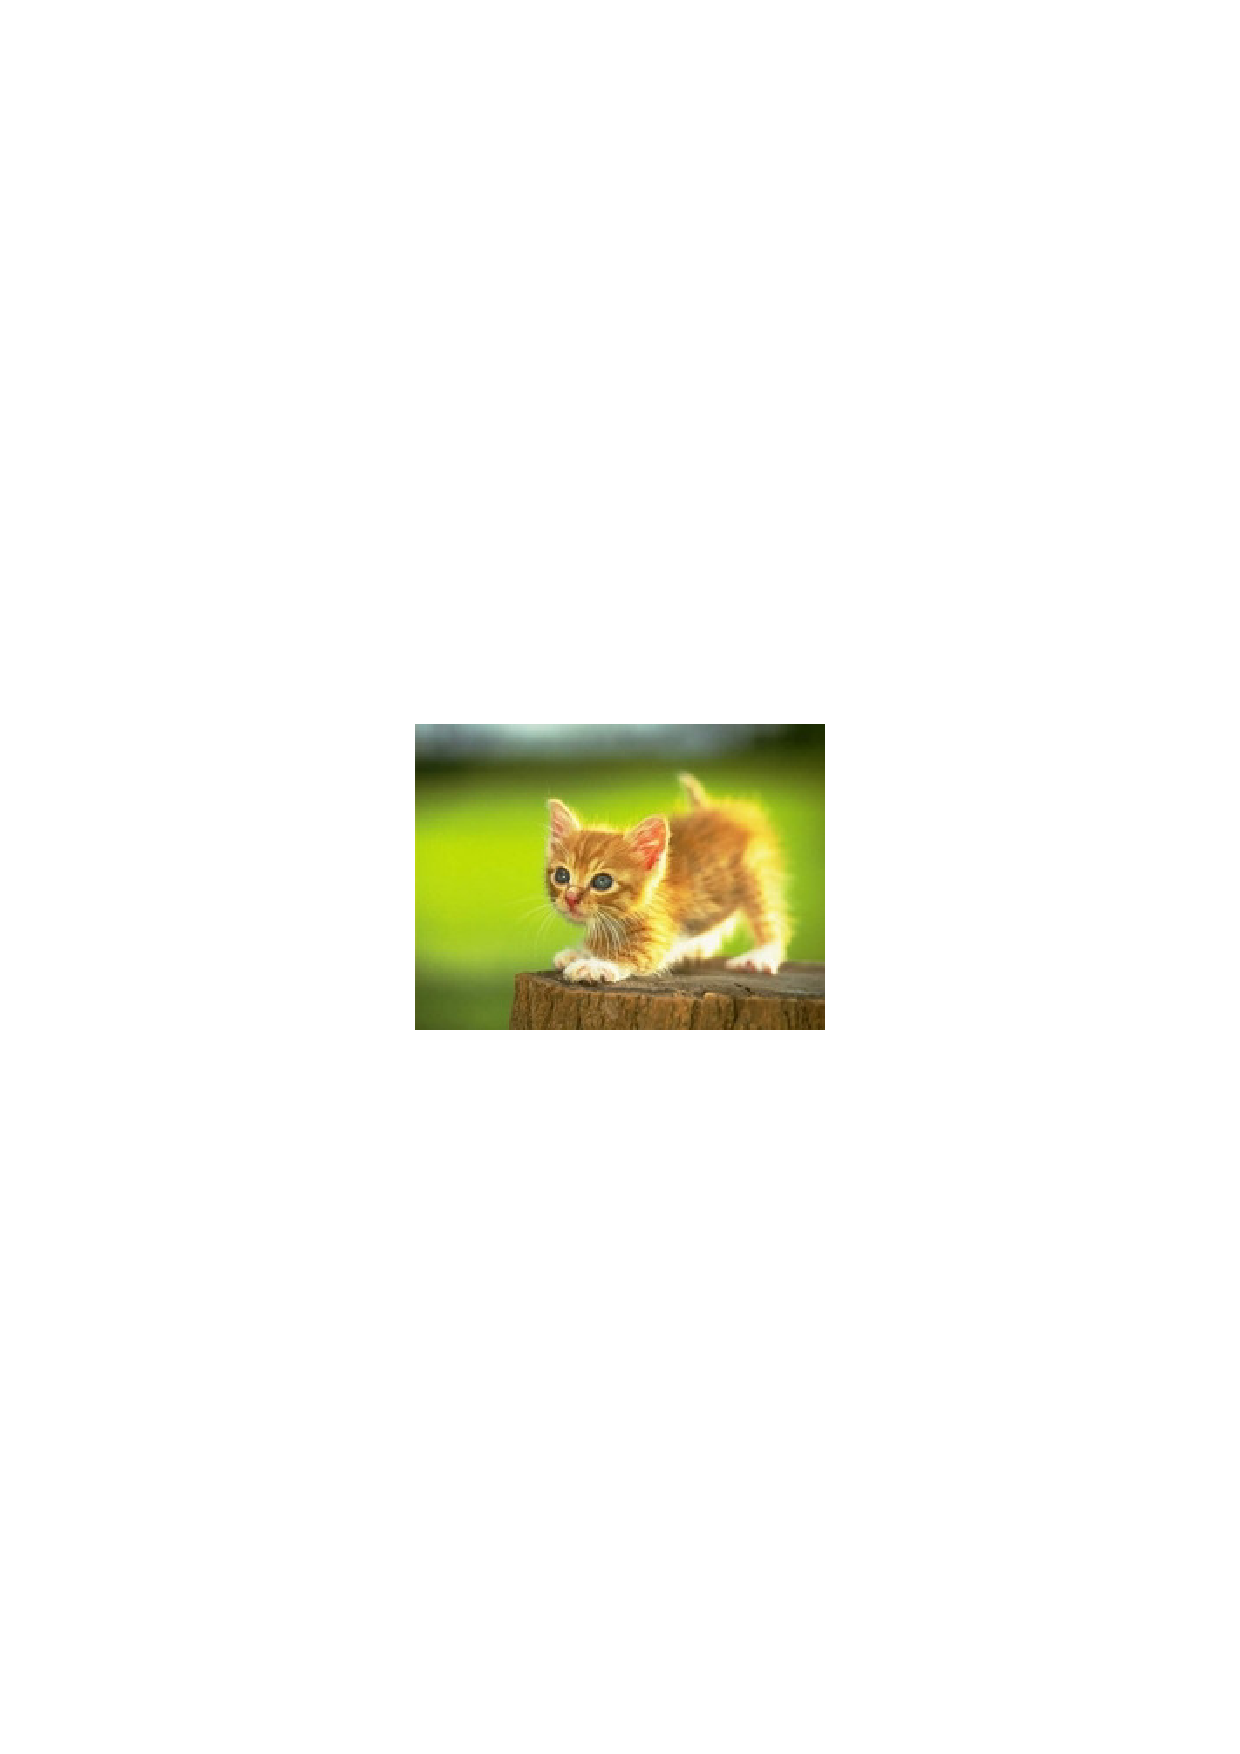
\includegraphics{cat}
\caption{一只猫的幸福}\label{fig:cat}
\end{figure}

四十年来家国,三千里地山河。 凤阁龙楼连霄汉,玉树琼枝作烟萝。
几曾识干戈。 一旦归为臣虏,沉腰潘鬓消磨。
最是仓皇辞庙日,教坊犹奏离别歌。 垂泪对宫娥。

是岁十月之望,步自雪堂,将归于临皋。二客从予过黄泥之坂。
霜露既降,木叶尽脱,人影在地,仰见明月,顾而乐之,行歌相答。
已而叹曰:“有客无酒,有酒无肴,月白风清,如此良夜何!”
客曰:“今者薄暮,举网得鱼,巨口细鳞,状如松江之鲈。顾安所得酒乎?”
归而谋诸妇。 妇曰:“我有斗酒,藏之久矣,以待子不时之需。”
于是携酒与鱼,复游于赤壁之下。江流有声,断岸千尺;山高月小,
水落石出。曾日月之几何,而江山不可复识矣。予乃摄衣而上,
履谗岩,披蒙茸,踞虎豹,登虬龙,攀栖鹘之危巢,俯冯夷之幽宫。
盖二客不能从焉。划然长啸,草木震动,山鸣谷应,风起水涌。予亦悄然而悲,
肃然而恐,凛乎其不可留也。反而登舟,放乎中流,听其所止而休焉。
时夜将半,四顾寂寥。适有孤鹤,横江东来。翅如车轮,玄裳缟衣,
戛然长鸣,掠予舟而西也。 须臾客去,予亦就睡。梦一道士,羽衣蹁跹,
过临皋之下,揖予而言曰:“赤壁之游乐乎?”问其姓名, 俯而不答。
“呜呼!噫嘻!我知之矣。畴昔之夜,飞鸣而过我者,非子也邪?”
道士顾笑,予亦惊寤。开户视之,不见其处。


\subsection{并排子图}

图~\ref{fig:cat1} 和~图~\ref{fig:cat2} 是位于浮动环境中的并列子图。
\begin{figure}[!htbp]%
\centering
\subfloat[一只猫的幸福]{\label{fig:cat1}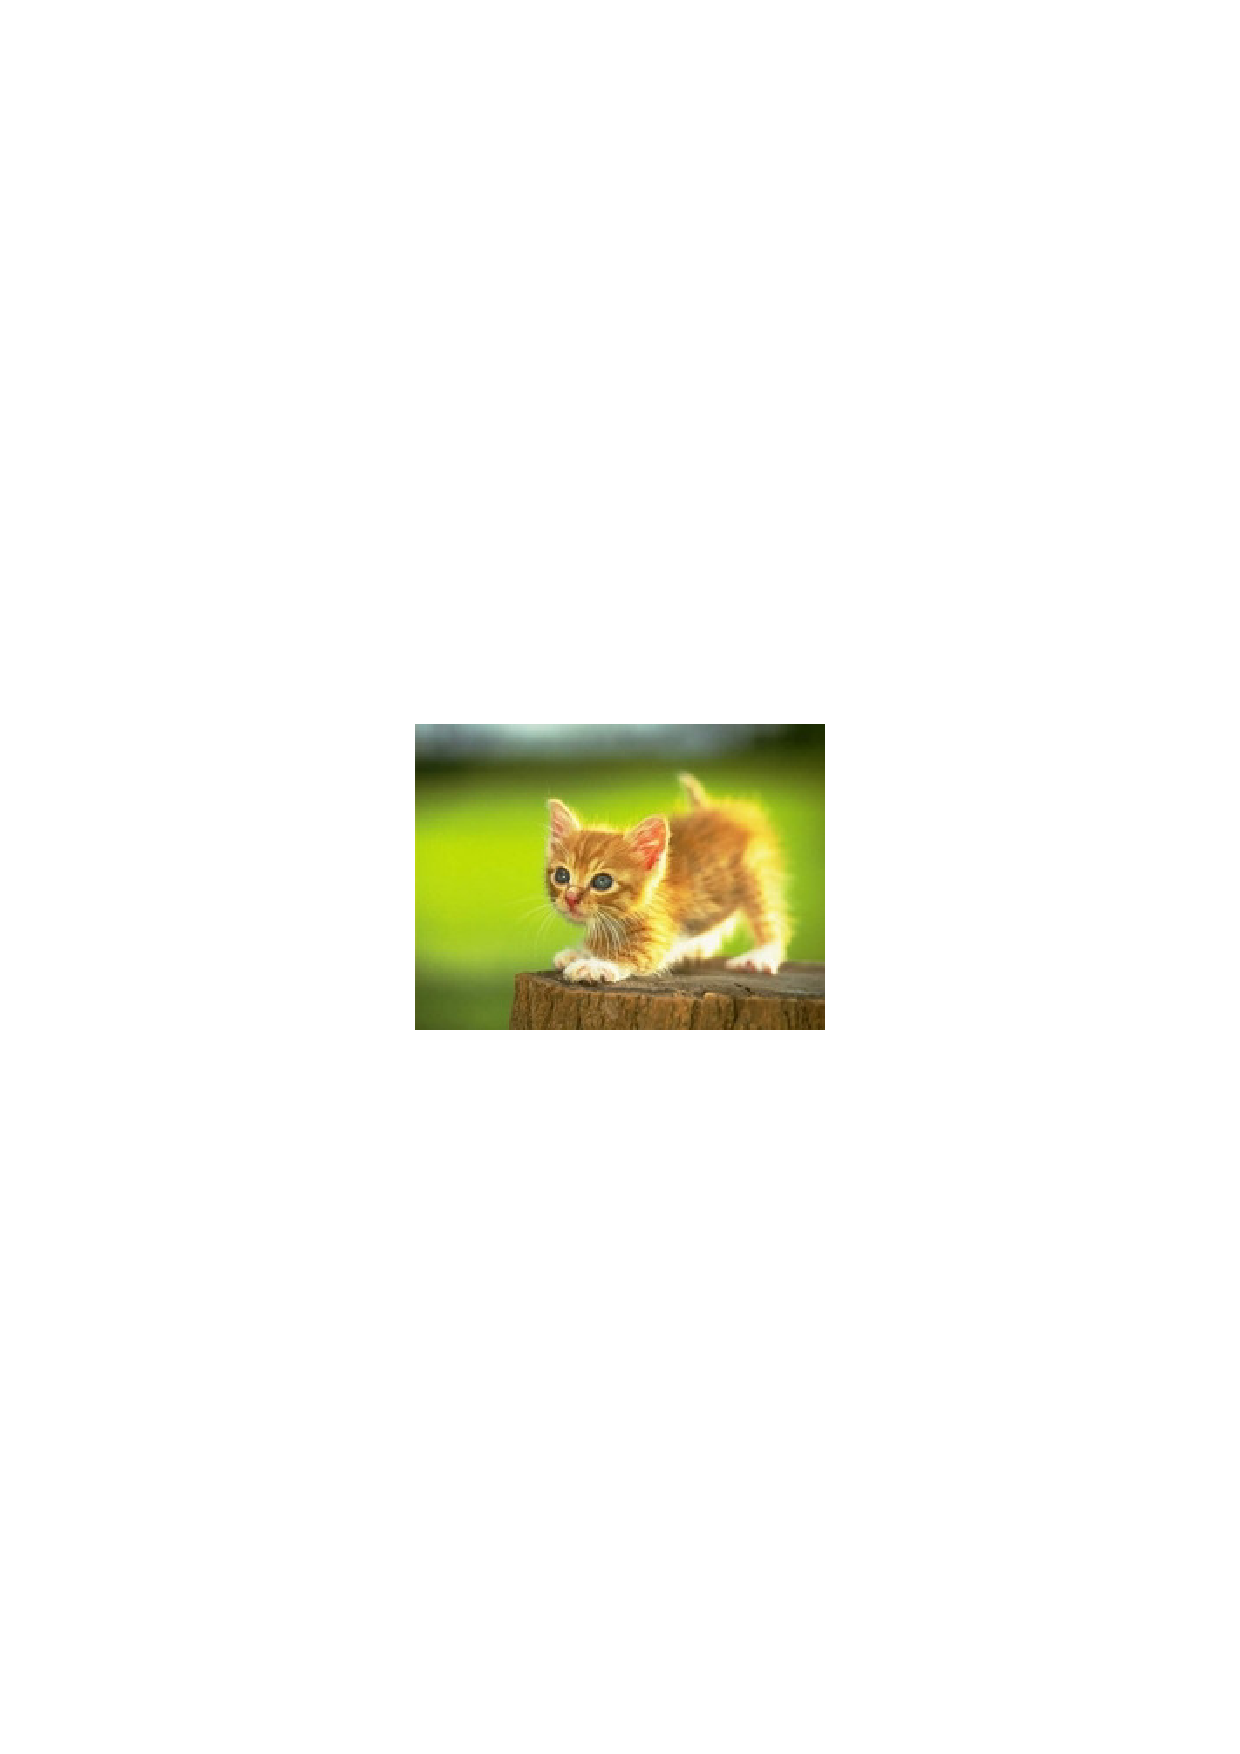
\includegraphics[scale=0.9]{cat}}%
\qquad
\subfloat[一只猫的幸福]{\label{fig:cat2}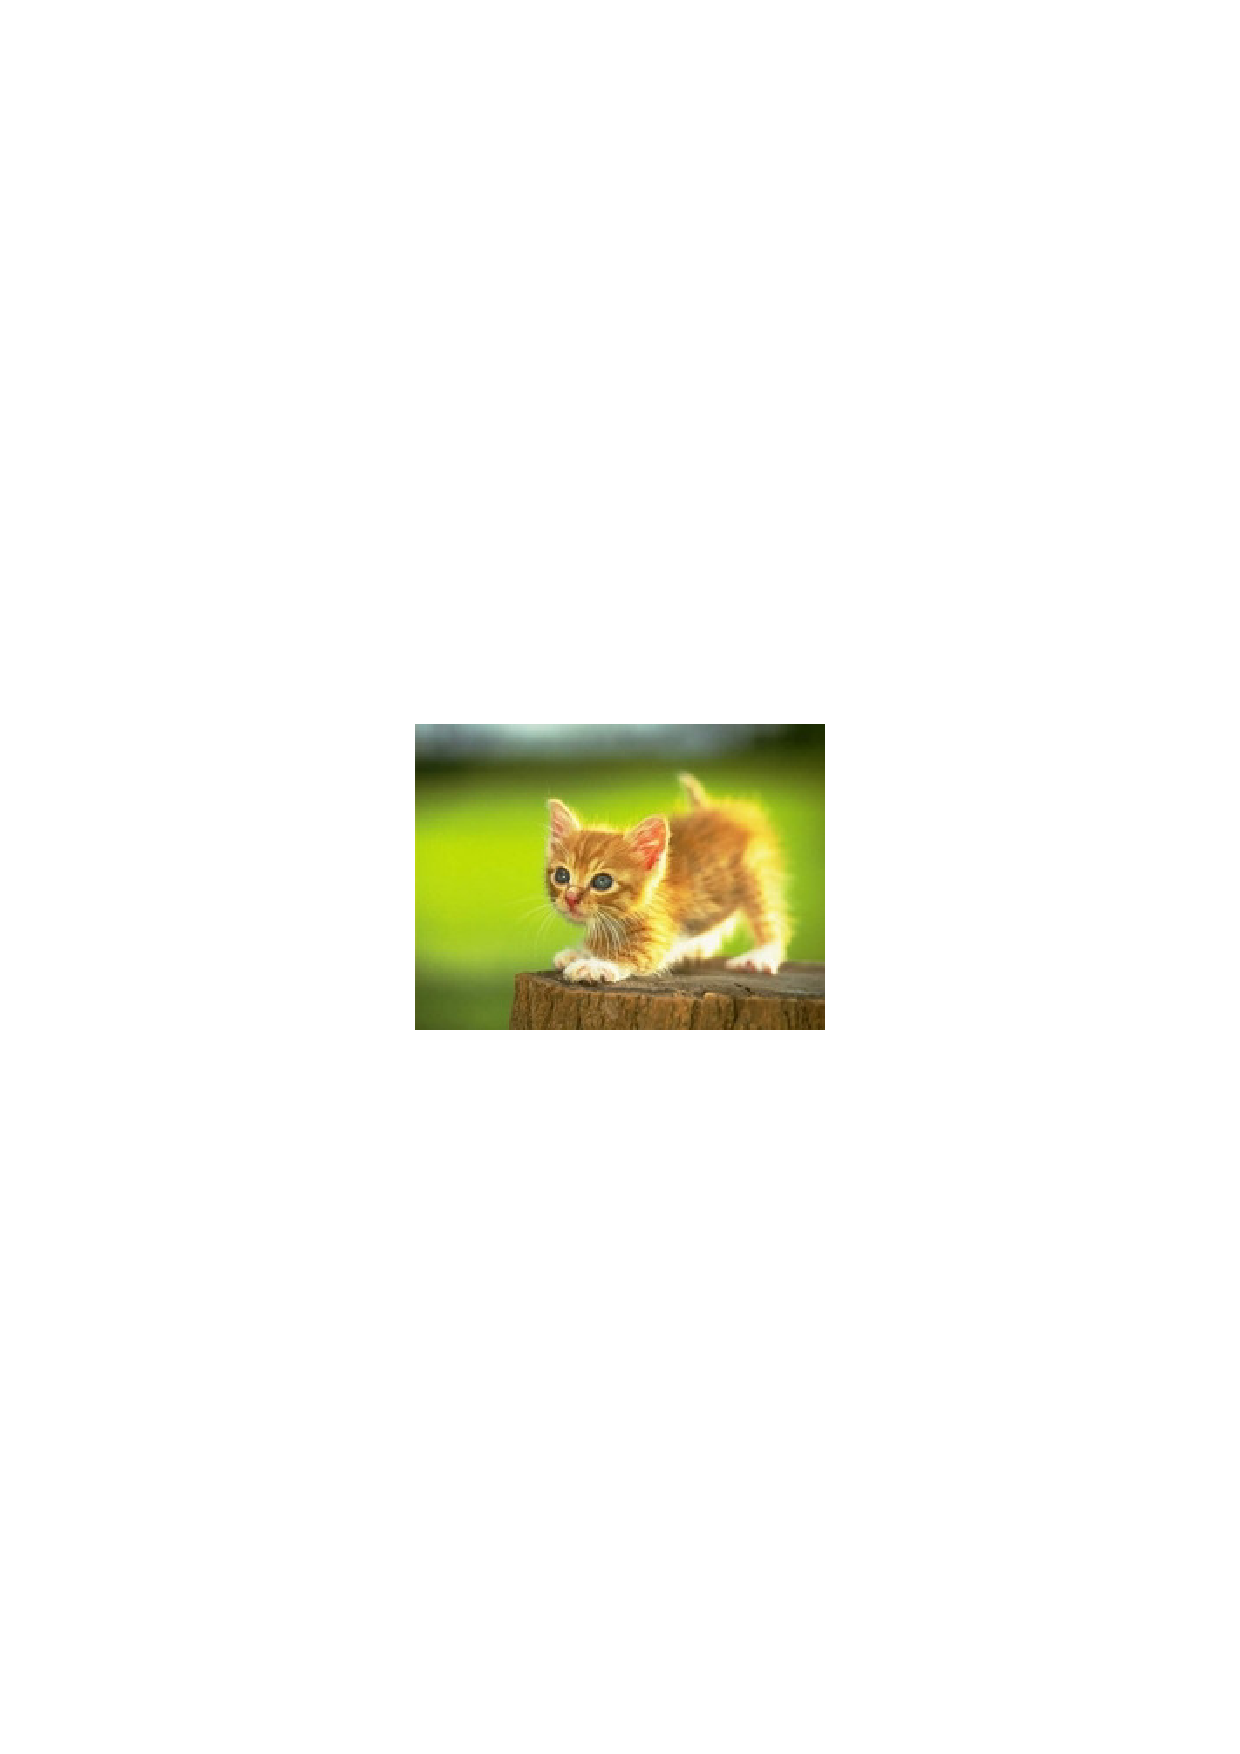
\includegraphics[scale=0.9]{cat}}%
\caption{A Tale of Two Kitties.}%
\end{figure}

月朦胧,鸟朦胧,点点萤火照夜空。 山朦胧,树朦胧,唧唧秋虫正呢哝。
花朦胧,叶朦胧,晚风轻轻叩帘栊。 灯朦胧,人朦胧,今宵但愿同入梦。

\chapter{实验研究类论文*}
\label{cha:thirdsection}


\section{引言(引言标题可选)}
\label{sec:method}
由于绪论中已对全文相关的研究背景和进展做了综述,因此,每章的引言中,请用1页左右的版面写一个导引,简要说明本章研究的背景或动机,以起到承上启下的作用,不宜太长。

引言的最后一段,说明本章的主要内容,如拟基于什么理论或方法,针对什么问题开展研究。注意:这里不能给结论。

若少于1个页面时,建议省略标题“引言”,直接在章的标题下写上几段话即可。

若学位论文属实验研究类论文,且论文所用的实验材料、仪器设备、实验方法基本一样,但应用不同,此时可考虑在第二章用整章的篇幅来描述,这样后面的章节就无需描重复描述相同内容,以避免冗余。

若实验性研究论文所用的材料与方法并非完全相同时,建议在各章中分别介绍材料与方法、实验结果、分析与讨论,最后是小结。



\section{材料与方法}
\label{sec:algorithm}

\subsection{实验材料}
针对材料的描述,一般应给出材料来源。

\subsection{实验仪器}
针对仪器的描述,若为商用仪器,给出型号、品牌、产地。

若为自行搭建的系统,则需要简要说明介绍组成及原理。

\subsection{实验方法}
介绍本章所涉及的实验方法或实验步骤。

\subsection{数据处理(根据情况确实是否需要)}
主要介绍对所获得的数据是如何处理的。

\section{结果1(请拟定具体的题目)}
作为章节的二级标题,若直接采用“结果与分析”,则在目录中看不到有效信息。为避免出现毫无辨识度的标题,建议将所得的结果作为二级标题,但也不要一幅图一节,将相关的结果整合为2-3节即可,各节篇幅长短不宜悬殊太大。

\section{结果2(请拟定具体的题目)}

\section{结果3(请拟定具体的题目)}

\section{分析与讨论}
论文排版时,无论因为图表等原因还是其它原因,除章与章的之间存在分页,空白处的地方不要太多。

讨论部分的关键在于:分析本章所得到的一些结果之间的关联性;所得到的结果与文献结果是否一致?分析产生一致或不一致结果的原因,以此体现论文的创新点。也可以指出本章中的不足,并分析原因及未来改进措施。

\section{本章小结}
本章主要介绍实验研究类的论文正文章节的框架结构。在每章的最后,都需要对该章的内容进行小结,不宜太长,建议1/2-2/3页版面较好。主要小结一下本章用什么理论或方法、做了什么事、得到的重要结果或结论。

\chapter{理论/算法类研究类论文}
\label{cha:fourthsection}



\section{引言(引言标题可选)}
\label{sec:parameters}
无论什么类型的论文,在章节的标题下,都需要简要说明本章研究的背景或动机,以起到承上启下的作用。若少于1个页面时,建议省略标题“引言”,直接在章的标题下写上几段话即可。

对于非会议、期刊的信息来源,若为网址,请在当页中脚注中加以标注*。

理论研究类论文,一般包括原理介绍、理论推导/或算法设计思想,再通过模拟仿真给出结果。该类论文若提出的是新理论或算法,一般应与现有理论/算法比较。当然也可以通过实验加以验证,以评估其准确性。具体内容应包括以下几个部分:


\section{理论/算法}

\section{仿真或算法实现}

\section{理论/算法准确性的评估}

\section{分析与讨论}

\section{本章小结}
本章简要给出理论/算法类研究论文的基本框架。在每章的最后,都需要对该章的内容进行小结,不宜太长,建议1/2-2/3页版面。主要小结一下本章用什么理论或方法、做了什么事、得到的重要结果或结论。


%%% 结论
%%% mode: latex
%%% TeX-master: t
%%% End:

\chapter{总结与展望}
\label{cha:conclusion}

\section{本文主要内容及结论}
\label{sec:conclusion}
对全文进行全面地总结,并根据各章节归纳出若干有机联系的论点。按正文的内容分段描述,包括本研究“做了什么(提出**新理论/算法、设计或研发**工艺/仪器)、获取什么结果、得出什么结论”。

请特别注意,全文总结与摘要及各章的小节要有所区分,不能简单的拷贝。这里的重点是结论,结论应该准确、完整、明确、精练。

\textcolor{red}{(论文总结与摘要及各章的小节有区分,不简单拷贝。总结包含学位论文的创新点。)}


\section{本文主要创新点}
\label{sec:contribution}
通常情况下,学位论文的创新点应放在最后一章。

创新点要凝炼,表述要清晰明了,如提出了什么创新的思路,主要特点是什么,相比现有理论或技术的提高是什么、或者有什么新的发现,是否具有重要的科学意义或应用前景。既不能过于简单,也不要太细。

硕士学位论文创新点不宜太多,一般为2个左右即可,要注意归纳创新点,千万不要以为越多越好。论文的创新不以创新点的多少来评定的,而以其创新性的价值来评定。几章的工作合在一起凝炼成一个创新点也不是不可以的。


\section{展望}
\label{sec:futurework}
对本研究成果的意义、推广应用的现实性或可能性加以论述。同时,描述本文研究中尚存在的不足,或因时间尚未完成但又必须继续的工作,对进一步的工作进行展望。

%%% 致谢

%%% Local Variables:
%%% mode: latex
%%% TeX-master: "../main"
%%% End:

\begin{ack}

这里写致谢。

\end{ack}



%%% 参考文献
%Included for Gather Purpose only:
%input "ref/refs.bib"
\bibliographystyle{HUSTThesis}
\bibliography{ref/refs}



%%% 附录(根据自己实际情况增加或删减)
\begin{appendix}
\chapter{答辩委员会决议}

\setlength{\baselineskip}{20pt}
{

首行缩进两个字符,中文字体采用小四宋体,英文字体采用Times New Roman,字体大小为小四,行间距为固定值20磅。

}
%% 根据自己实际情况增加或删减
\begin{publications}
\noindent
\textbf{发表与接收论文}
\renewcommand{\labelenumi}{[\arabic{enumi}]}
\begin{enumerate}
    \item 参照参考文献列出学术论文相关信息(含期刊、会议、或参编书稿),但无论有多少个作者,都必须列出全部作者名;若为英文论文,则名在前姓在后,姓名均为全称;在本人的名字加粗,以示区别(若为第一作者,则需在最后特别注明署名华中科技大学是否为第一单位)
    \item 若已发表,按参考文献给出页码;若只是online,给出链接;若接受或修改或投稿或拟投,也必须分别注明
    \item 一般情况,一作或重要的论文放在前面
    \item Hajiali, Faezeh, \textbf{Saeid Tajbakhsh}, and Akbar Shojaei. Fabrication and properties of polycaprolactone composites containing calcium phosphate-based ceramics and bioactive glasses in bone tissue engineering: a review[J]. Polymer Reviews, vol. 58, no. 1, pp. 164-207, 2018.(SCI源刊;IF:5.375;署名单位:华中科技大学)
\end{enumerate}
\vspace{2em}
\textbf{专\hspace{2em}利}
\renewcommand{\labelenumi}{[\arabic{enumi}]}
\begin{enumerate}
    \item 全部作者的姓名全称,本人的名字加粗. 专利题名. 专利国别,专利文献种类,专利号或申请号
\end{enumerate}
\vspace{2em}
\textbf{标\hspace{2em}准}
\renewcommand{\labelenumi}{[\arabic{enumi}]}
\begin{enumerate}
    \item 全部作者的姓名全称,本人的名字加粗. 标准题名. 哪种层次的标准,发表年
\end{enumerate}
\vspace{2em}
\textbf{科技奖励}
\renewcommand{\labelenumi}{[\arabic{enumi}]}
\begin{enumerate}
    \item 全部作者的姓名全称,本人的名字加粗. 题目. 国家级/省部级科技类奖,获奖年
    \item 全部作者的姓名全称,本人的名字加粗. 题目. 国际/国内竞赛类奖,获奖年
\end{enumerate}
\end{publications}

\chapter{公开发表的学术论文与博士学位论文的关系}
\begin{center} 
\song \xiaosi
%\vspace{2.0cm}
\renewcommand{\arraystretch}{1.5}
\begin{longtable}{|p{0.9cm}<{\centering}|p{2.8cm}<{\centering}|p{2.4cm}<{\centering}|p{3cm}<{\centering}|p{4cm}<{\centering}|}
    \hline
    \makecell{序号}&\makecell[c]{成果名称}&\makecell[c]{成果形式}&\makecell[c]{成果主要内容}&\makecell[c]{与学位论文对应的关系}\\
    \hline
    1&\makecell[c]{}
    & \makecell[c]{}
    & \makecell[c]{}
    & \makecell[c]{}\\
    \hline
    2&\makecell[c]{}
    & \makecell[c]{}
    & \makecell[c]{}
    & \makecell[c]{}\\
    \hline
    3&\makecell[c]{}
    & \makecell[c]{}
    & \makecell[c]{}
    & \makecell[c]{}\\
    \hline
    4&\makecell[c]{}
    & \makecell[c]{}
    & \makecell[c]{}
    & \makecell[c]{}\\
    \hline
    5&\makecell[c]{}
    & \makecell[c]{}
    & \makecell[c]{}
    & \makecell[c]{}\\
    \hline
\end{longtable}
\end{center}  

%\chapter{攻读博士学位期间参与的科研项目}
\begin{project}
\renewcommand{\labelenumi}{\textbf{\arabic{enumi}.}}
   \begin{enumerate}
    \item   \textbf{项目类型}\\  
            项目名称: 项目名称 \\
            项目编号: No. 88888888 \\
            起止时间: 2018年8月至2018年8月 \\
            担任角色:担任角色 \\
   \end{enumerate}
\end{project} 
\chapter{中英文缩写对照表}
\begin{center} \xiaosi
%\vspace{2.0cm}
\renewcommand{\arraystretch}{1.5}
\begin{tabular}{p{2.3cm}p{12.7cm}}
    3D&Three-dimensional(三维)\\
    CT&Computer tomography (计算机断层层析成像)\\
    MRI&Magnetic resonance imaging(磁共振成像)\\
    PET&Positron emission computed tomography(正电子发射断层成像)\\
    …&
\end{tabular}
\end{center}  
\chapter{其它数据图表或程序}
\end{appendix}

\end{document}
